\chapter{Vector Calculus}  

\section{Vector Fields}   
So far we have been studying calculus of \textit{functions} of several
variables.   In this chapter we look at \emph{vector fields,} we will learn
the meaning of their derivatives, and we'll see how to integrate them.

By definition, a vector field in the plane is a vector valued function:
whereas an ordinary function of two variables gives you a number for each
$(x, y)$ in its domain, a vector field gives you a vector in the plane
for each point $(x,y)$ in its domain.   Such a vector is determined by its
two components, both of which are ordinary functions of $(x, y)$.   The
notation we will use in 234 is as follows:
\begin{equation}
  \vv(x, y) = \vek P(x, y) \\ Q(x, y)\tor = 
  P(x,y) \vi + Q(x, y) \vj.
  \label{eq:05vectorfield-notation}
\end{equation}
Vector fields in three dimensional space are similar: at each point if for
each point $(x, y, z)$ in a domain you specify a vector $\vv(x, y, z)$,
then you have defined a 3D vector field:
\[
\vv(x, y) = \vek P(x, y) \\ Q(x, y) \\ R(x, y)\tor = 
P(x,y) \vi + Q(x, y) \vj + R(x, y)\vk.
\]
To draw a vector field in the plane you would have compute $\vv(x, y)$ at
lots of points and simply plot them.   The more points you pick, the busier
the picture gets.   See for example Figure~\ref{fig:05grad-theta}, in which
the vector field
\begin{equation}\label{eq:05grad-theta}
  \vv(x, y) = \vek -y / (x^2+y^2)\\ x/(x^2+y^2) \tor
\end{equation}
is drawn.

We have already seen examples of vector fields before, namely the gradient
of any function $f(x, y)$ is a vector field:
\[
\nab f(x, y) = \vek f_x(x, y) \\ f_y(x, y)\tor.
\]
In fact, the example (\ref{eq:05grad-theta}) is such a vector field: it is
the gradient of the polar angle $\theta$.  For $x>0$ this angle is given by
$\theta(x, y)$, and you checked in problem \ref{prb:grad-of-theta} that
$\vv$ given by (\ref{eq:05grad-theta}) satisfies $\vv = \nab \theta$.
\begin{figure}[t]
  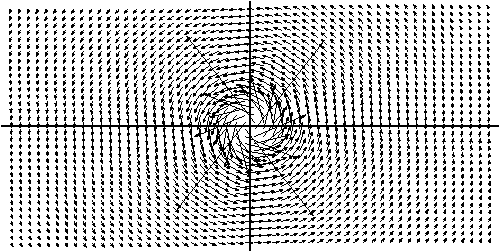
\includegraphics[scale=1]{figures/05vectorfield.pdf}
  \caption{\textbf{A vector field in the plane.}  This vector field is
    $\vv(x, y) = \nab \theta(x, y) = \frac{-y}{x^2+y^2}\vi +
    \frac{x}{x^2+y^2}\vj$.   In general, drawings of vector fields become
    messy in the region where the vectors are long, because they tend to
    overlap.   Drawing a three dimensional vector field is challenging.}
  \label{fig:05grad-theta}
\end{figure}


\section{Examples of vector fields}  

\subsection{Fluid flow}\label{sec:fluid-flow}  
Vector fields appear in various ways in physics.   The easiest way to
visualize a vector field is by thinking of it as the velocity field of a
fluid flow.   Suppose a fluid is flowing through a certain region in space.
The velocities of the fluid particles will generally vary from place to
place, and also with time.   A fluid flow is called \textit{steady} if the
velocity of a fluid particle only depends on its location.   This means that
the velocity vector $\vv$ of a fluid particle is a function of its
coordinates $(x, y, z)$ only, and does not depend on time.

For instance, if a viscous fluid flows through a cylindrical pipe, the
velocity of the fluid will only depend on the distance to the central axis
of the pipe.   On the walls the velocity will vanish (the fluid sticks to
the wall of the pipe), and in the center the fluid will move fastest.
Under certain circumstances it follows from the laws of fluid mechanics
that the velocity field (1) is always parallel to the central axis, and (2)
depends quadratically on the distance to the central axis:
\begin{equation}
  \label{eq:05poisseuille-flow}
  \vv(x, y, z) = v_c\, \bigl(1-\frac{r^2} {R^2}\bigr)\vi
  = \vek v_c \bigl(1-(r/R)^2\bigr) \\ 0\\0\tor ,
\end{equation}
where $R$ is the radius of the pipe, $r$ is the distance to its central
axis, and $v_c$ is the velocity at the center of the pipe.

This example describes a the motion of a fluid, but a vector field can be
the velocity field of anything that moves, in particular, a gas flow has a
velocity field, and the velocities in a moving elastic solid (think
``Jello'') must also be described by a vector field.

\begin{figure}[hb]
  \centering
  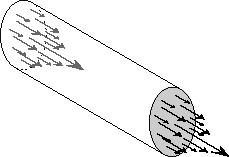
\includegraphics{figures/05poiseuille3D.pdf}\qquad
  \begin{picture} (200.000000,105.125000)(0,0)
    \put(0.0, 0.0){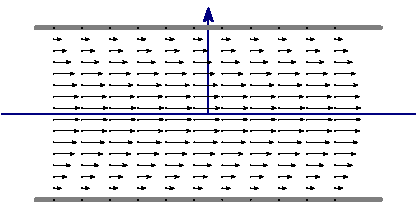
\includegraphics{05poiseuille.pdf}}
        \put(182.50,  52.50){\sffamily\itshape central axis}
    \put(104.00,  95.88){\sffamily\itshape $r$}
    \put(184.50,  89.88){\sffamily\itshape wall}

\end{picture}

  \caption{\textbf{Fluid flow in a cylindrical pipe.  } \textbf{Left: } as a
    viscous fluid flows through a pipe it sticks to the walls, and so its
    velocity will be highest at the center of the pipe.  \textbf{Right: } a
    drawing of a cross section the flow on the left.   We see the vector
    field corresponding to so-called \textit{Poiseuille flow,} given by
    Equation~(\ref{eq:05poisseuille-flow}).}
  \label{fig:05poisseuille-flow}
\end{figure}

\subsection{Force fields}   
If we assume the Earth is flat, then the gravitational force it exerts on a
mass $m$ is always the vector $\vF = \tvek 0 \\ -mg\ttor$.   We can think of
this as a constant vector field: its magnitude and direction are the same
everywhere.

But the Earth is not flat, and according to Newton the gravitational force
$\vF$ is a vector pointing towards the center of the earth, whose magnitude
is inversely proportional to the distance to the center of the Earth.   If
we choose the Earth's center to be the origin, then Newton's law looks like
this:
\begin{equation}
  \label{eq:05Newton-on-gravity}
  \vF(x, y, z) = -C \frac{\vx}{\|\vx\|^3}, \qquad \vx = \vek x\\y\\z\tor.
\end{equation}
\marginpar{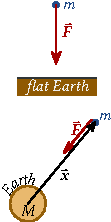
\includegraphics[scale=1.25]{figures/05newtons-law.pdf}}%
Here $C$ is a constant which depends on the masses $m$ of the object, and
$M$ of the Earth (in physics books one finds that $C= GMm$, where $G$ is
called the ``universal gravitational constant.'')

Other prominent examples of vector fields appear in the theory of
electromagnetism.   The electric currents and charges around us create an
electric field and a magnetic field, which at each point in space are given
by vectors $\vE$ and $\vB$.   These vectors change from place to place, and
so they define vector fields
\[
\vE = \vE(x, y, z), \qquad \vB=\vB(x, y, z).
\]
For example, Coulomb's law states that the electric field generated by a
charged particle at the origin is given by
\begin{equation}
  \label{eq:05coulombs-law}
  \vE(x, y, z) = \frac{Q} {4\pi\epsilon_0} \frac{\vx} {\|\vx\|^3},
\end{equation}
which is almost the same as Newton's law (\ref{eq:05Newton-on-gravity}) for
the gravitational field.   Here $\epsilon_0$ is some constant, and $Q$ is the
electric charge of the particle.

If an electric current of strength $I$ runs upward through the $z$-axis,
then this current will create a magnetic field which is given by
\begin{equation}
  \label{eq:05field-of-current}
  \vB(x, y, z) = \frac{\mu_0 I} {2\pi}
  \vek -y/(x^2+y^2) \\ x/(x^2+y^2) \\ 0 \tor.
\end{equation}
Again, a constant ($\mu_0$) appears.   If you compare
(\ref{eq:05field-of-current}) with (\ref{eq:05grad-theta}), then you will
notice that, except for the constant factor $\mu_0 I /2\pi$ this vector
field is a three dimensional version of the one drawn in
Figure~\ref{fig:05grad-theta}: you can regard Figure~\ref{fig:05grad-theta}
as a ``top view'' of the magnetic field $\vB$ of an electric current.
\marginpar{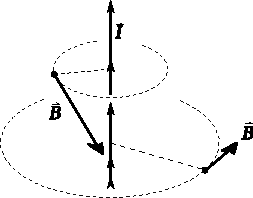
\includegraphics[scale=0.8]{figures/05magneticfield.pdf}}

\section{$\nab$ -- differentiating vector fields}  
\label{sec:nabla}
The components of a vector field are functions, and therefore you can
differentiate them.   Various combinations of the partial derivatives of
vector fields turn out to be very useful, and to appear in the natural
world.   The easiest way to describe these is to introduce the so-called
``nabla operator'' (or ``del operator'') defined by
\begin{equation}
  \nab =  \vek \pdd{}x\\[2pt] \pdd{}y \\[2pt] \pdd{}z\tor =
  \pdd{}x\vi +  \pdd{}y \vj + \pdd{}z \vk.
\end{equation}
At first sight something is missing here: there are partial derivatives,
but the function whose derivative is supposed to be taken is missing.   This
is intentional, and the way $\nab$ is to be interpreted is as follows:
\begin{center}
  \itshape
  in any formula containing $\nab$,\\
  the partial derivatives are to be taken of\\
  all functions appearing to the \emph{right} of the $\nab$.
\end{center}
For example, if $f(x, y, z)$ is a function of $(x,y,z)$, then
\[
\nab f
=\vek \pdd{}x\\[2pt] \pdd{}y \\[2pt] \pdd{}z\tor\;f(x, y, z)
=\vek\pdd fx(x, y, z) \\[2pt]\pdd fy(x, y, z) \\[2pt] \pdd fz(x, y, z)\tor.
\]
So $\nab f$ is the gradient of the function $f$, just as we had defined it
before.   Sometimes a different notation is used, namely
\[
\nab f = \grad f.
\]

Next, supposing you have a vector field
\[
\vv = \vek P(x, y, z)\\Q(x, y, z)\\R(x, y, z) \tor
\]
what would be the result of ``multiplying'' $\nab$ with $\vv$?  Since we
think of $\nab$ as a vector, the multiplication can be either a dot
product, or a cross product.   If you ``take the dot product'' of $\nab$ and
$\vv$, you get
\[
\nab \dpp \vv
= \vek \pdd{}x\\[2pt] \pdd{}y \\[2pt] \pdd{}z\tor
 \dpp \vek P \\ Q \\ R\tor
= \pdd Px + \pdd Qy + \pdd Rz.
\]
Other commonly used notation for the divergence is
\[
\div \vv  = \nab\dpp\vv.
\]
This combination of derivatives of the components of $\vv$ is called the
\emph{divergence of the vector field} $\vv$.

If you take the cross product of $\nab$ and $\vv$ you find the so-called
\emph{curl of the vector field} $\vv$,
\[
\nab \cp \vv =
\left|
  \begin{matrix}
    \vi & \pdd{}x & P \\[2pt]
    \vj & \pdd{}y & Q \\[2pt]
    \vk & \pdd{}z & R
  \end{matrix}
  \right|
  =\vek R_y - Q_z\\ P_z - R_x \\ Q_x - P_y\tor.
\]
The curl of a vector field $\vv$ is sometimes called the ``rotation of
$\vv$,'' and the following alternative notations also get used:
\[
\nab \cp \vv = \curl \vv = \rot \vv.
\]

\subsection{Example -- compute the divergence of $\vv(x, y, z) = \vx$ and  
  $\vw = \rho\vx$}
\label{sec:divx-and-divrhox}
The vector fields are
\[
\vv(x, y, z) = \vx = \vek x\\y\\z\tor,
\text{ and }
\vw(x, y, z) = \rho\vx = \vek \rho x\\\rho y \\ \rho z\tor,
\]
in which $\rho$ is the radius from spherical coordinates, i.e.
\[
\rho = \sqrt{x^2+y^2+z^2}.
\]
The divergence of $\vv$ is easy:
\[
\nab\dpp\vv = \pdd xx + \pdd yy + \pdd zz = 3, \text{ or } \div \vv =3.
\]
The divergence of $\vw$ is a little harder.   To begin with, you have
\[
\nab\dpp\vw = \pdd{\rho x}x + \pdd{\rho y}y + \pdd{\rho z}z.
\]
It helps to find the partial derivatives of $\rho$ separately.   They are
\[
\pdd \rho x = \frac{x} {\rho},\qquad
\pdd \rho y = \frac{y} {\rho},\qquad
\pdd \rho z = \frac{z} {\rho}.
\]
These formulas look nicer in vector form, namely
\begin{equation}\label{eq:05gradient-of-rho}
  \nab \rho = \vek x/\rho\\y/\rho\\z/\rho\tor
  =\frac{1} {\rho}\vek x\\y\\z\tor = \frac{\vx} {\rho}.
\end{equation}
(Problem \ref{prb:gradrho-and-divx} will ask you to check this.)  Armed
with these partial derivatives we find
\[
\pdd{\rho x}x = \frac{x} {\rho}x + \rho \pdd xx = \frac{x^2} {\rho} + \rho.
\]
You get similar terms for $\pdd{\rho y}y$ and $\pdd{\rho z}z$.   Adding
these together leads to
\[
\nab\dpp\vw
= \frac{x^2} {\rho} +\frac{y^2} {\rho} +\frac{z^2} {\rho} +3\rho
= \frac{x^2 + y^2 + z^2} {\rho} +3\rho
= \frac{\rho^2} {\rho} + 3\rho
= 4\rho.
\]

\subsection{Example -- compute the curl of the Poiseuille flow from  
  \S~\ref{sec:fluid-flow}}
The flow is given in Equation (\ref{eq:05poisseuille-flow}).   For
simplicity we will assume $R=1$ and $v_c=1$.   If we assume that the central
axis is the $x$ axis, then the distance $r$ to the central axis is
$r=\sqrt{y^2+z^2}$, and the velocity field in the cylinder is given by
\[
\vv(x, y, z) = \vek 1-y^2 - z^2 \\0 \\0 \tor.
\]
Its curl is then
\[
\nab\cp\vv
=
\left|
  \begin{matrix}
    \vi & \pdd{}x &  1-y^2 - z^2 \\
    \vj & \pdd{}y & 0 \\
    \vk & \pdd{}z & 0
  \end{matrix}
\right|
=
\vek 0 \\ -2z \\ +2y \tor
\]

\subsection{The curl of a gradient always vanishes}  
\label{sec:curl-of-grad-is-zero}
If $f(x, y, z)$ is any function of three variables, then its gradient is a
vector field.   What is the curl of this vector field?  The computation is
straightforward,
\begin{equation}
  \nab\cp\nab f
  =
  \nab\cp \vek f_x\\ f_y\\ f_z\tor
  =\left|
    \begin{matrix}
      \vi & \pdd{}x &  f_x \\
      \vj & \pdd{}y &  f_y \\
      \vk & \pdd{}z & f_z
    \end{matrix}
  \right|
  =\vek (f_z)_y - (f_y)_z\\(f_x)_z - (f_z)_x \\ (f_y)_x - (f_x)_y\tor.
  \label{eq:05compute-curl-of-grad}
\end{equation}
We know that for any function of several variables ``mixed partials are
equal'' (when they are continuous), meaning $(f_x)_y = (f_y)_x$, etc.
Another look at the curl we just computed tells us that
\begin{equation}
  \label{eq:curl-of-grad-is-zero}
  \nab\cp\nab f = \vvv0, \text{ or, }
  \curl\grad f = \vvv0,
\end{equation}
for any function $f$ (whose second derivatives are continuous).

\subsection{The divergence of a curl always vanishes}  
\label{sec:div-of-curve-is-zero}
A computation just like the one above shows that if you have a vector field
$\vv$ and you compute the divergence of its curl, you always get zero:
\begin{equation}
  \label{eq:div-of-curl-is-zero}
  \nab\dpp(\nab\cp\vv) = 0, \text{ or, }
  \div \curl \vv = 0.
\end{equation}
Both Equations (\ref{eq:curl-of-grad-is-zero}) and
(\ref{eq:div-of-curl-is-zero}) are easy to remember in their ``$\nab$''
form, if you pretend that $\nab$ is a real vector.

To get (\ref{eq:curl-of-grad-is-zero}) remember that the cross product of
any vector with itself always vanishes: $\va \cp \va =\vvv0$ for any $\va$.
The expression $\nab\cp\nab f$ contains the cross product of $\nab$ with
itself, and so it should vanish.   The argument doesn't hold because $\nab$
is not really a vector, but our computation
(\ref{eq:05compute-curl-of-grad}) shows that the conclusion is true anyway.

To get (\ref{eq:div-of-curl-is-zero}), you use that $\va\cp\vb$ is always
perpendicular to $\vb$, no matter what $\va$ and $\vb$ are, so that
$\va\dpp(\va\cp\vb) = 0$ always holds.   Equation
(\ref{eq:div-of-curl-is-zero}) is exactly that, with ``$\va = \nab$'' and
``$\vb = \vv$.''

\begin{figure}[t]
  \centering\framebox{
    \begin{minipage}[c]{0.7\textwidth}
      \vspace{3pt}
      \[
      \text{function} \stackrel{\grad}\longrightarrow \text{vector field}
      \stackrel{\curl}\longrightarrow \text{vector field}
      \stackrel{\div}\longrightarrow \text{function}
      \]
      \[
      f \stackrel{\grad}\longrightarrow \nab(f) \cdots\cdots \vv
      \stackrel{\curl}\longrightarrow \nab\cp \vv \cdots\cdots \vw
      \stackrel{\div}\longrightarrow \nab\dpp\vw
      \]
      \vspace{0.1ex}
    \end{minipage}}
  \caption{The three basic operations of vector calculus.   If you apply two
    consecutive operations in this diagram, you get zero.   See Equations
    (\ref{eq:curl-of-grad-is-zero}) and (\ref{eq:div-of-curl-is-zero}).}
\end{figure}
\subsection{Other combinations of gradient, curl and divergence} 
The divergence of the gradient does not normally vanish.   If you expand the
definitions you find
\[
\nab\dpp\nab f =
\frac{\pd^2 f} {\pd x^2} +\frac{\pd^2 f} {\pd y^2} +\frac{\pd^2 f} {\pd z^2}.
\]
This combination of second derivatives of a fuction, which occurs very
often is called the \emph{Laplacian} of the function $f$.   The following
notation is used:
\[
\triangle (f) = \nab\dpp\nab f = f_{xx} + f_{yy} + f_{zz}.
\]


\section{Problems}  
\problemfont
\begin{multicols}{2}
\problem If the central axis of the cylinder in 
Figure~\ref{fig:05poisseuille-flow} is the $x$-axis, and if the vector
field is as given in (\ref{eq:05poisseuille-flow}), then write $\vv$ in
terms of $x, y, z$ instead of $r$.
\answer The distance to the central axis is $r^2 = y^2+z^2$, so
\[
\vv(x, y, z) = v_c\, \bigl(1-\frac{y^2+z^2} {R^2}\bigr)\vi
\]
\endanswer
\problem Show that the magnetic field in (\ref{eq:05field-of-current}) can 
be written as
\[
\vB(x, y, z) = C \frac{\vk\cp\vx} {\|\vk\cp\vx\|^n}
\]
for some integer $n$ and some constant $C$.   Find the right $n$ and $C$.
\answer
$n=2$ and $C=\mu_0 I/2\pi$.
\endanswer
\problem \label{prb:05derivs-of-a-times-m-dot-x} 
Let $\va$ and $\vm$ be two constant vectors, with components
\[
\va = \tvek a_1\\a_2\\a_3\ttor, \text{ and }
\vm = \tvek m_1\\m_2\\m_3\ttor.
\]
Let $\vv(x, y, z)$ be the vector field $\vv = (\vm\dpp\vx)\va$.

\subprob Write $\vv$ in terms of its components:
\[
\vv = \tvek \cdots?\cdots \\ \cdots?\cdots \\ \cdots?\cdots \ttor.
\]
\subprob Compute $\nab\dpp \vv$.  

\subprob Compute $\nab \cp \vv$.  

\subprob If $\vv$ is the gradient of some function $f$, 
what can you say about the vectors $\va$ and $\vm$?

\subprob If $\vv$ is the curl of some vector field $\vw$, 
what can you say about the vectors $\va$ and $\vm$?

\problem \label{prb:05derivs-of-a-exp-of-mx} 
Let $\va$ and $\vm$ be as in the previous problem.
Consider the vector field
\[
\vv(x, y, z) = e^{\vm\dpp\vx}\va = e^{m_1x+m_2y+m_3z}\tvek a_1\\a_2\\a_3\ttor.
\]

\subprob Show by computing the derivatives 
that $\nab \bigl(e^{\vm\dpp\vx}\bigr) = e^{\vm\dpp\vx} \vm$.
\answer
$\bigl(e^{\vm\dpp\vx}\bigr)_{x_1} = m_1e^{\vm\dpp\vx}$, and the same for the $x_2$
and $x_3$ derivatives.   Therefore
\[
\nab\bigl(e^{\vm\dpp\vx}\bigr) =
\vek m_1e^{\vm\dpp\vx}\\m_2e^{\vm\dpp\vx} \\ m_3e^{\vm\dpp\vx} \tor
=e^{\vm\dpp\vx} \tvek m_1\\m_2\\m_3\ttor.
\]
\endanswer
\subprob Compute $\nab\dpp \vv$.   (Find the shortest way to write 
the answer.)
\answer
After simplifying you get $\nab\dpp\vv = \vm\dpp\va e^{\vm\dpp\vx}$.
\endanswer
\subprob Compute $\nab\cp\vv$.\label{prb:05cross-prod-of-aexpmx} 
Again, simplify your answer.
\answer
$\nab\cp\vv = \vm\cp\va e^{\vm\dpp\vx}$.
\endanswer
\subprob Which condition must the vectors $\va$ and $\vm$ satisfy if  
$\vv$ is to be ``divergence free,'' i.e.\ if $\div \vv = 0$?
\answer
$\va$ and $\vm$ must be perpendicular.
\endanswer
\subprob Suppose that $\vv = \nab \phi$ for some function.  
What do you know about $\va$ and $\vm$?
\answer
If $\vv$ is the gradient of some function, then its curl must vanish.
Therefore $\va\cp\vm=\vvv0$ in view of part \ref{prb:05cross-prod-of-aexpmx}
of this problem.   The conclusion is that $\va$ and $\vm$ must
be parallel.
\endanswer
\problem If $\vv=\tvek P\\ Q \\ R\ttor$ is a vector field and $f$ is 
a function, then what is $\vv\dpp\nab f$?
\answer
$\vv\dpp\nab f = P f_x + Q f_y + R f_z$.
\endanswer
\problem \emph{Product rules.  }\label{prb:05product-rule} 
Let $f$ be a function of three variables, and let $\vv$ be a three
dimensional vector field.

\subprob $\nab\dpp(f\vv) = (\nab f)\dpp\vv + f \nab\dpp\vv$ 
\answer
By definition,
\begin{align*}
  \nab\dpp(f\vv) = \nab \dpp \vek fP\\fQ \\fR\tor
  &= \pdd{fP}x + \pdd{fQ}y + \pdd{fR}z  \\
  &= f_x P + fP_x + f_yQ + fQ_y + f_z R + fR_z\\
  &= f_x P +f_y Q + f_z R + f\bigl(P_x+Q_y+R_z\bigr) \\
  &= \vek f_x\\ f_y\\ f_z\tor \dpp \vek P\\Q\\R\tor + f \nab\dpp\vv \\
  &= \nab f\dpp \vv + f\nab \dpp\vv,
\end{align*}
as claimed.
\endanswer
\subprob Guess a product rule for $\nab\cp(f\vv)$ and prove it.  
\answer
$\nab\cp(f\vv) = (\nab f)\cp\vv + f\nab\cp\vv$ is the rule.
The derivation goes along the same lines as in the previous product rule.
\endanswer
\problem \label{prb:gradrho-and-divx} Check the following 
formulas
\[
\nab \rho = \frac{\vx} {\rho}, \text{ and }
\nab\dpp \vx = 3.
\]
\answer
This is example~\ref{sec:divx-and-divrhox}.
\endanswer

\problem Use the product rule from Problem~\ref{prb:05product-rule} and 
the formulas from problem \ref{prb:gradrho-and-divx} to compute the
following quantities

\subprob $\nab\dpp(\rho^2\vx)$ 
\answer
$5\rho^2$.
\endanswer
\subprob $\vx\dpp\nab\rho$ 
\answer
$\vx\dpp\frac\vx\rho= \|\vx\|^2/\rho = \rho^2/\rho = \rho$.
\endanswer
\subprob $\DS \div \frac{\vx} {\|\vx\|^3}$.   What does this say 
about the Earth's gravitational field?
\answer
Note that $\|\vx\| = \rho$, so you have to compute $\nab\dpp(\vx/\rho^3)$.
The answer is zero.

It says that the divergence of the gravitational field of the Earth is zero.

\endanswer



\problem \label{prb:x-no-curl} 
In this problem, as in all the problems in this section,
$\rho = \sqrt{x^2+y^2+z^2} = \|\vx\|$
is the radius in spherical coordinates.

\subprob Show that $\vx = \frac12 \nab(\rho^2)$.  

\subprob Compute $\nab\cp\vx$ without doing any derivatives.  
\answer
Since $\vx$ is the gradient of some function its curl must vanish.
\endanswer
\subprob Compute $\nab\cp(\rho\vx)$ using the product rule from 
problem \ref{prb:05product-rule}.
\answer
$\nab\cp(\rho\vx) = (\nab \rho)\cp \vx + \rho \nab\cp\vx = \vvv0$
\endanswer
\problem Compute $\nab\cp\vv$ for the vector field 
$\vv(x, y, z) = \vk\cp\vx$.
\answer
$\vv(x, y, z) = \tvek -y \\x \\ 0\ttor$
so $\nab\cp\vv = \tvek 0\\0\\2\ttor = 2\vk$.
\endanswer
\problem\label{prb:05div-rho-n-x} Consider the vector field
\[
\vv(x, y, z) = \rho^n \vx,
\]
where $n$ is a constant.   (Both Newton's law of gravitation
and Coulomb's law have this vector field with $n=-3$.)

\subprob Write $\vv(x, y, z)$ in the form $\tvek \cdots\\\cdots\\\cdots\ttor$, 
using only Cartesian coordinates $x, y, z$.
\answer
$\vv(x, y, z) =
\vek
   x(x^2+y^2+z^2)^{n/2} \\ y(x^2+y^2+z^2)^{n/2} \\ z(x^2+y^2+z^2)^{n/2}
\tor$.
\endanswer


\subprob Compute $\nab\dpp\vv$.   (Use one of the product 
rules from Problem \ref{prb:05product-rule}; you can also
avoid computing the derivatives of $\rho$ by looking them
 up in the text.)
\answer
Using the product rule, you get
\[
\nab(\rho^{-n}\vx)
= (\nab \rho^{-n})\dpp\vx + \rho^{-n}\nab\dpp\vx
= -n\rho^{-n-1}(\nab\rho)\dpp\vx + \rho^{-n}\nab\dpp\vx.
\]
Now recall (or compute again):
\[
\nab \rho = \frac{\vx} {\rho}, \text{ and }
\nab\dpp\vx = 3.
\]
This leads to
\[
\nab(\rho^{-n}\vx)
= - n \rho^{-n-1}\frac{\vx} {\rho}\dpp\vx + 3 \rho^{-n}
= - n \rho^{-n-2}\|\vx\|^2 + 3 \rho^{-n}
= (-n+3) \rho^{-n})
\]
\endanswer
\subprob For which value(s) of $n$ does one have $\div \vv = 0$? 
\answer
$n=3$.
\endanswer
\problem\label{prb:05grad-Frho} A function of three variables
is called \emph{radially symmetric}
if it only depends on the radius $\rho = \sqrt{x^2+y^2+z^2}$, i.e.\
if it can be written as $F(\rho)$ for some function $F$ of one variable.
E.g.\ $f(x, y, z) = \rho^{-2}$, or $g(x, y, z) = e^{-\rho}$ are radially
symmetric functions.  

\noindent%
\textit{Find the gradient of a radially symmetric function $F(\rho)$.}

(You may want to use $\rho_x = x/\rho$, etc.~from (\ref{eq:05gradient-of-rho})
to speed up the computation.)
\answer
There are a long and a short answer.  
The long(er) computation goes likes this:
\[
\nab F(\rho)
= \vek F(\rho)_x\\ F(\rho)_y \\ F(\rho)_z\tor
= \vek F'(\rho)\rho_x\\ F'(\rho)\rho_y \\ F'(\rho)\rho_z\tor
= F'(\rho)\vek \rho_x\\\rho_y\\\rho_z\tor.
\]
Now recall (\ref{eq:05gradient-of-rho}), and you find
\[
\nab F(\rho)
=F'(\rho)\vek x/\rho\\y/\rho\\z/\rho\tor
=\frac{1} {\rho}F'(\rho) \vx.
\]
The short computation is essentially the same, but you never
write the components of the vectors:
\[
\nab F(\rho) = F'(\rho) \nab \rho = \frac{1} {\rho}F'(\rho)\vx.
\]
\endanswer
\subprob Let $\vv = \rho^n\vx$, as in problem ref{prb:05div-rho-n-x}.  
Does there exist a function $f(x, y, z)$ such that $\vv = \nab f$?
(Hint: try a radially symmetric function, and use problem
\ref{prb:05grad-Frho}.)
\answer
If $f(x, y, z)= F(\rho)$, then by the previous problem
we have $\nab f = \rho^{-1}F'(\rho) \vx$.   We want this to be equal to
$\rho^{-n}\vx$, so $F(\rho)$ must satisfy
\[
\rho^{-1}F'(rho) = \rho^{n} \implies
F'(\rho) = \rho^{1+n} \implies
F(\rho) = \frac{\rho^{2+n}} {2+n} +C
\]
for some constant $C$.   We are only asked to find on function $f$,
so we find that the given vector field is indeed the gradient of a radially
symmetric function:
\[
\vv = \rho^{n}\vx = \nab \bigl(\frac{\rho^{2+n}} {2+n}\bigr).
\]
The exceptional case is when $n=-2$, in which case you get
$F(\rho) = \ln \rho$.
\endanswer

\end{multicols}
\noproblemfont


